\section{Apply Referring Expression Segmentation into Retrieval System}
The interactive retrieval system allows users to search for relevant images by inputting a language query. The system then retrieves matching images from the database, which usually contains the objects or concepts referred to in the query. This retrieval system and referring expression segmentation task uses both the text query and images as input. This shared input helps us to leverage the referring segmentation in our retrieval system, providing explainability and reliability in the retrieval results.

In our retrieval system, when a query is sent, the system responds with a rank-list of relevant images almost instantly. However, our referring expression segmentation module is not too fast (18 FPS). Therefore, to enhance the user experience, we leverage the text query to precisely point out the target object or concept referred to in the images that belong to the rank-list only.

Figure \ref{fig:res_retrieval_system} illustrates the using referring segmentation in our retrieval system for the explainability. It can be seen that the results are promising. With the query "a man next to the whiteboard", our system retrieves several images containing a man and a whiteboard next to him.
In most of the images, we successfully segment the person who stands right next to a whiteboard. In other cases, which contain no people in the images, our module even points out the whiteboard instead of a human, which is a reasonable replacement.


\begin{figure}[!t]
    \centering
    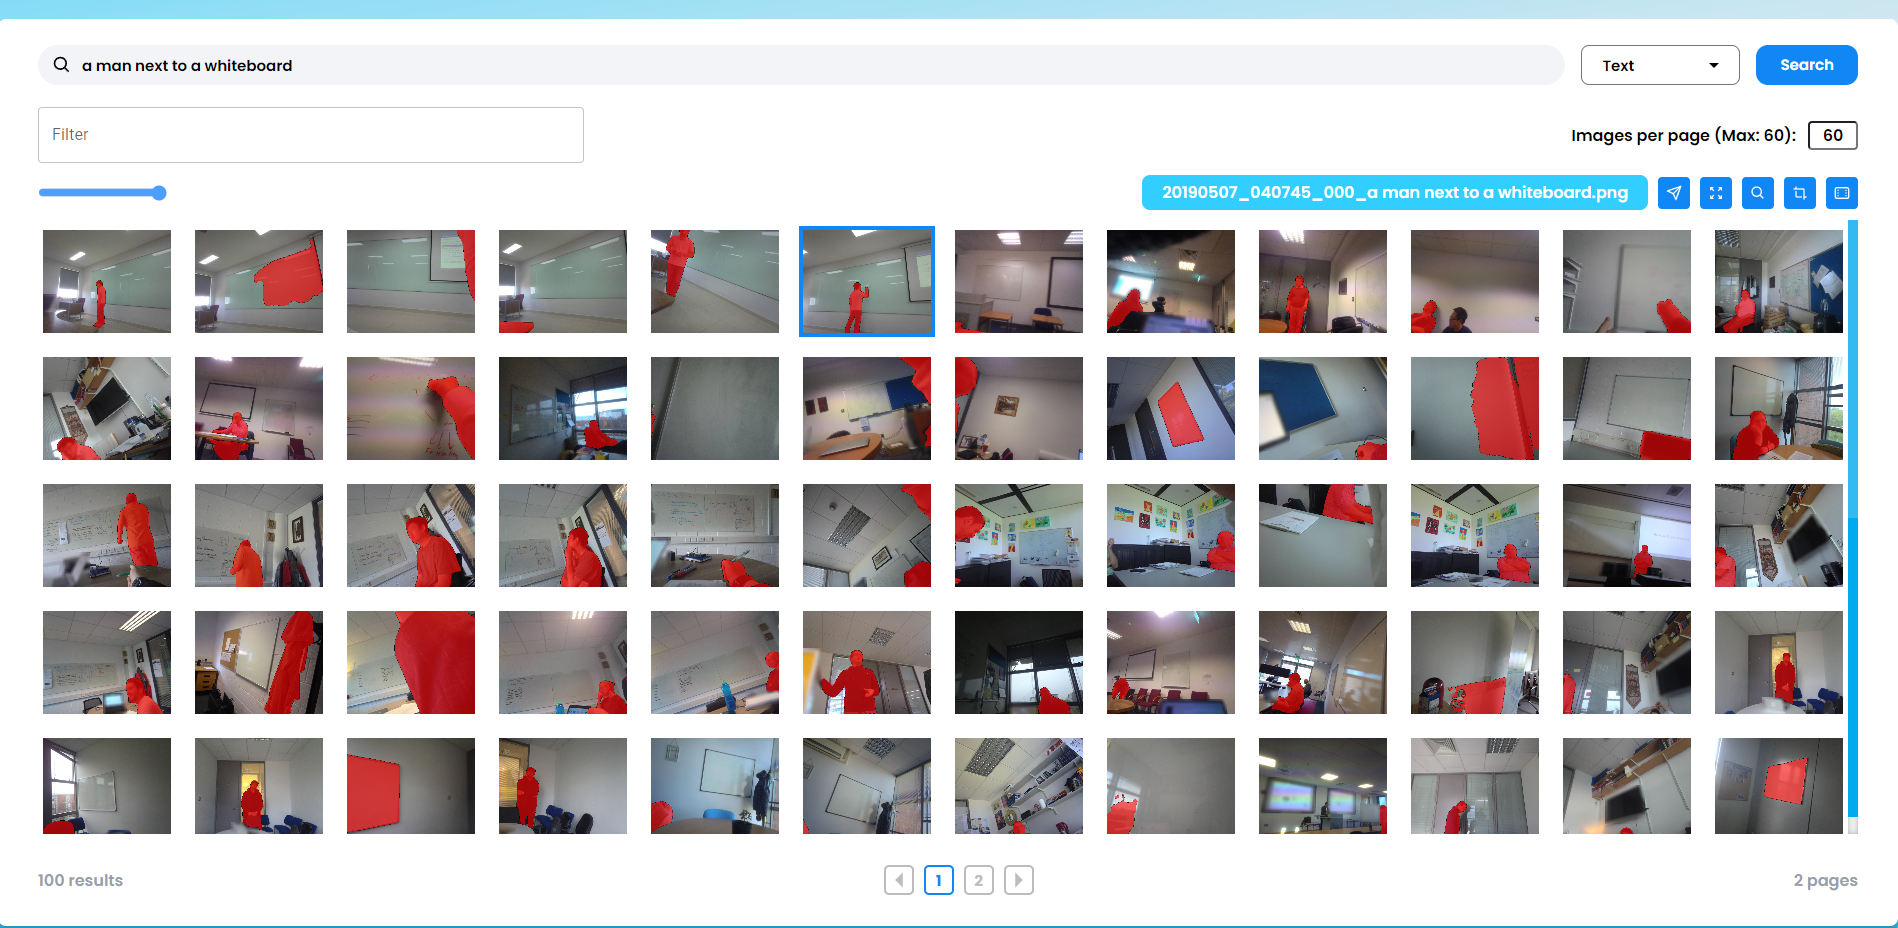
\includegraphics[width=0.8\linewidth]{content/resources/images/referring_segmentation/ReferringSegmentationInRetrievalSystem.png}
    \caption{An example of using referring expression segmentation in our retrieval system for the explainable retrieval results. The referred object is highlighted in the retrieval results in red color.}
    \label{fig:res_retrieval_system}
\end{figure}

